\setcounter{chapter}{11}
\chapter{Teste 1 2012/13}
\section{Pergunta 1}
\begin{equation*}
	f(x)=x^3+2x^2+10x-17
\end{equation*}
\begin{center} 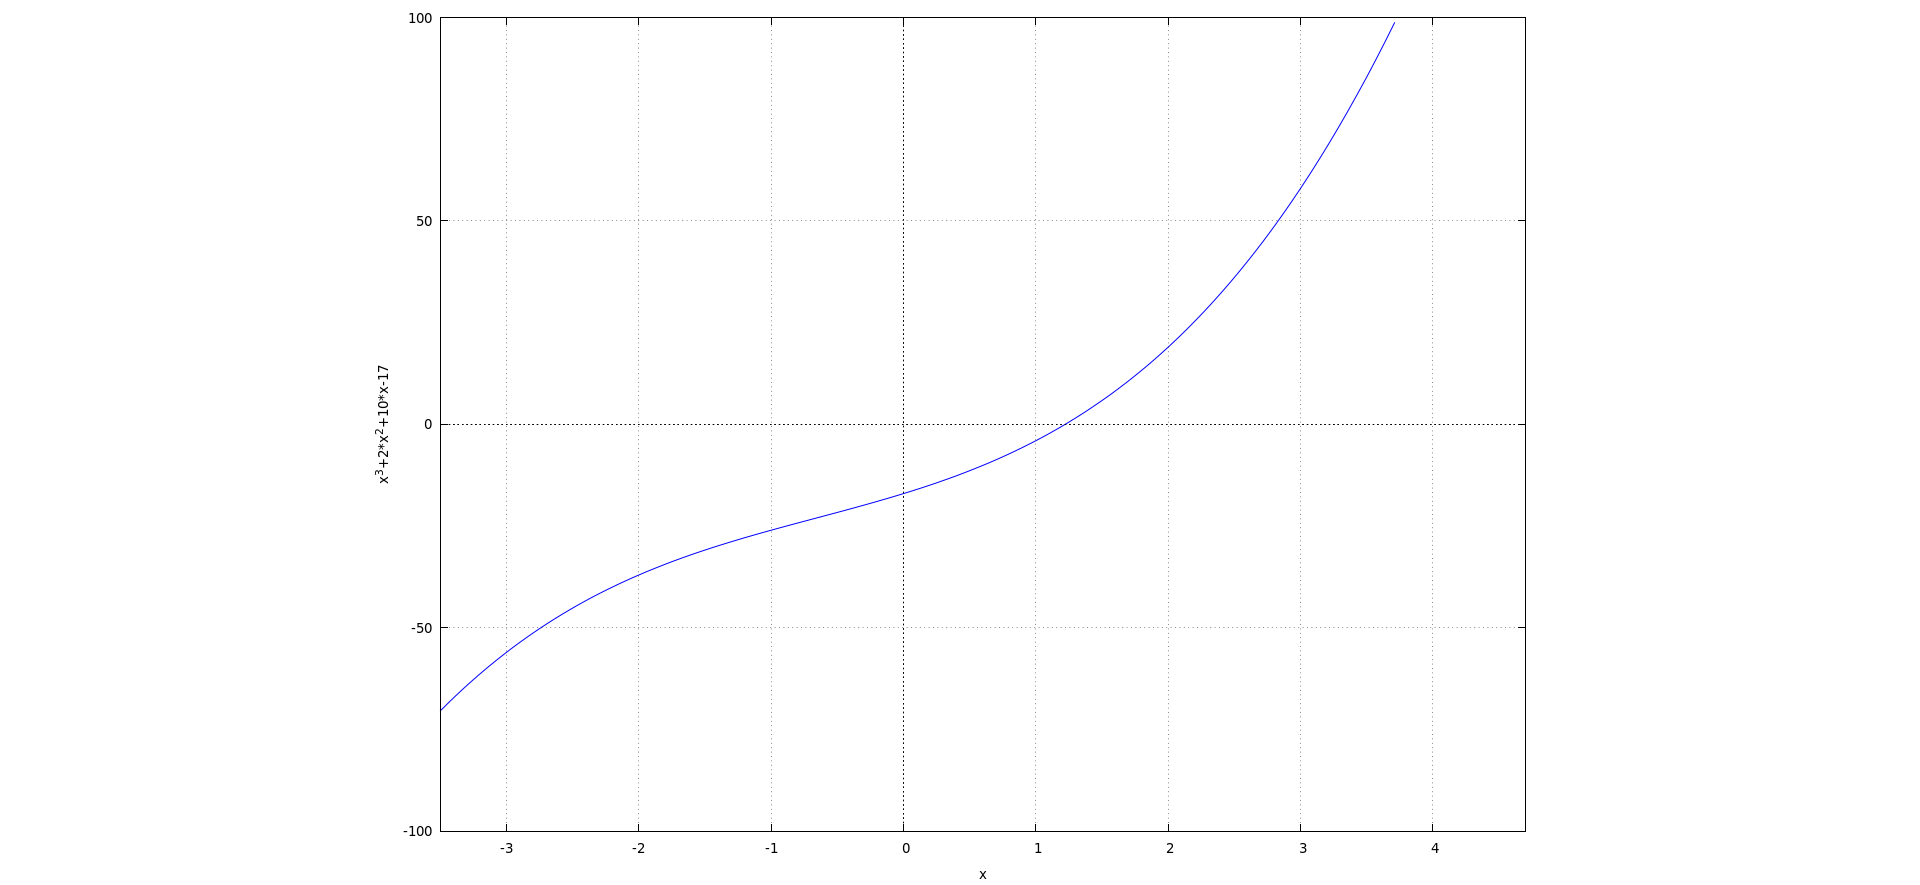
\includegraphics[height=65mm,keepaspectratio]{plot2012T1-1} \end{center}
Evidentemente, a maior raiz real de $f$ pertence ao intervalo $[-1.4, 2.6]$.
\section{Pergunta 5}
\begin{alignat*}{2}
	f(x) &=x^3+2x^2+10x-17\\
	f'(x)&=3x^2+4x+10\\
	g(x) &=x-\frac{f(x)}{f'(x)}\\
	     &=x-\frac{x^3+2x^2+10x-17}{3x^2+4x+10}\\
	     &=\frac{2x^3+2x^2+17}{3x^2+4x+10}\\
	x_{n+1} &\leftarrow g(x_n) 
\end{alignat*}
Utilizando uma folha de cálculo, os valores para as três primeiras iterações são:
\begin{center}
\begin{tabular}{c}
	$x_n$ \\ \hline
	0.0000 \\
	1.7000 \\
	1.2802
\end{tabular}
\end{center}

\section{Pergunta 6}
\begin{alignat*}{2}
	\begin{cases}
		f_1(x,y)=y-\ln(x-1)\\
		f_2(x,y)=y^2+(x-a)^2-r^2
	\end{cases}
	&\implies
	\mathbf{J}=\begin{bmatrix}
  		f_{1,x}' & f_{1,y}'\\
  		f_{2,x}' & f_{2,y}'
	\end{bmatrix}=\begin{bmatrix}
  		-(x-1)^{-1} & 1\\
  		2(x-a)      & 2y
	\end{bmatrix}\\
	&\implies
	|\mathbf{J}|=-2(x-a)-\frac{2y}{x-1}
\end{alignat*}
\begin{alignat*}{4}
	h&=-\frac{
		\begin{vmatrix}
			f_1 & f_{1,y}' \\
			f_2 & f_{2,y}'
		\end{vmatrix}}
		{|\mathbf{J}|}
	   &&=-\frac{
		\begin{vmatrix}
			y-\ln(x-1)      & 1 \\
			y^2+(x-a)^2-r^2 & 2y
		\end{vmatrix}}
		{|\mathbf{J}|}
	   &&=\frac{-y^2+2y(y-\ln(x-1))-(x-a)^2+r^2}{|\mathbf{J}|}\\
	k&=-\frac{
		\begin{vmatrix}
			f_{1,x}' & f_1 \\
			f_{2,x}' & f_2
		\end{vmatrix}}
		{|\mathbf{J}|}
	   &&=-\frac{
		\begin{vmatrix}
			-(x-1)^{-1} & y-\ln(x-1)      \\
			2(x-a)      & y^2+(x-a)^2-r^2
		\end{vmatrix}}
		{|\mathbf{J}|}
	   &&=\frac{\dfrac{y^2+(x-a)^2-r^2}{x-1}+2(x-a)(y-\ln(x-1))}{|\mathbf{J}|}
\end{alignat*}
\begin{equation*}
	\begin{cases}
		x'=x+h\\
		y'=y+k
	\end{cases}
\end{equation*}
\begin{lstlisting}[language=Maxima, caption=Comandos 2012T1-6 (MAXIMA)]
a : 3 $
r : 2 $
f1: y-log(x-1) $
f2: y^2+(x-a)^2-r^2 $
J : jacobian([f1,f2],[x,y]) $
J_: determinant(J) $
Ah: matrix([f1,diff(f1,y)],[f2,diff(f2,y)]) $
Ak: matrix([diff(f1,x),f1],[diff(f2,x),f2]) $
h : -determinant(Ah)/J_ $
k : -determinant(Ak)/J_ $
g1: x+h $
g2: y+k $
x0: 1.5;
y0: 1.3;
x1: subst([x=x0,y=y0],g1);
y1: subst([x=x0,y=y0],g2);
x2: subst([x=x1,y=y1],g1);
y2: subst([x=x1,y=y1],g2);
\end{lstlisting}
\begin{center}
\begin{tabular}{c | c}
	$x_n$   & $y_n$   \\ \hline
	1.50000 & 1.30000 \\
	3.8828  & 4.0725  \\
	6.3185  & 1.9037 
\end{tabular}
\end{center}
